\section*{Introdução}

A aeronave estudada neste trabalho é o Cirrus SR22, um avião ligeiro de asa baixa
com quatro a cinco lugares, fabricado pela Cirrus Aircraft (EUA) e utilizado
sobretudo em viagens privadas e na formação de pilotos. Deriva do SR20, que
realizou o primeiro voo a 21 de março de 1995~\cite{wiki_sr20}, e é produzido
desde 2001~\cite{wiki_sr22}. Em Portugal, a Nortávia (Maia, Porto) é um centro
certificado de formação e manutenção Cirrus, com formação de transição e
recorrente dirigida a proprietários e pilotos destes
aviões~\cite{afm_nortavia,flyingengineer_nortavia}.

A forma em planta da asa apresenta-se na Figura~\ref{fig:sr22} e as principais
dimensões na Tabela~\ref{tab:sr22}. A asa é afilada e tem alongamento elevado
(aspect ratio $AR \approx 10{,}1$). Segundo o \emph{Incomplete Guide to Airfoil Usage}~\cite{lednicer}, a asa
usa na raiz e na ponta um perfil Roncz, desenhado por John Roncz especificamente
para a Cirrus, cujas coordenadas não estão publicadas. Como indicado no
enunciado, utiliza-se o perfil da raiz como referência.

\begin{figure}[H]
  \centering
  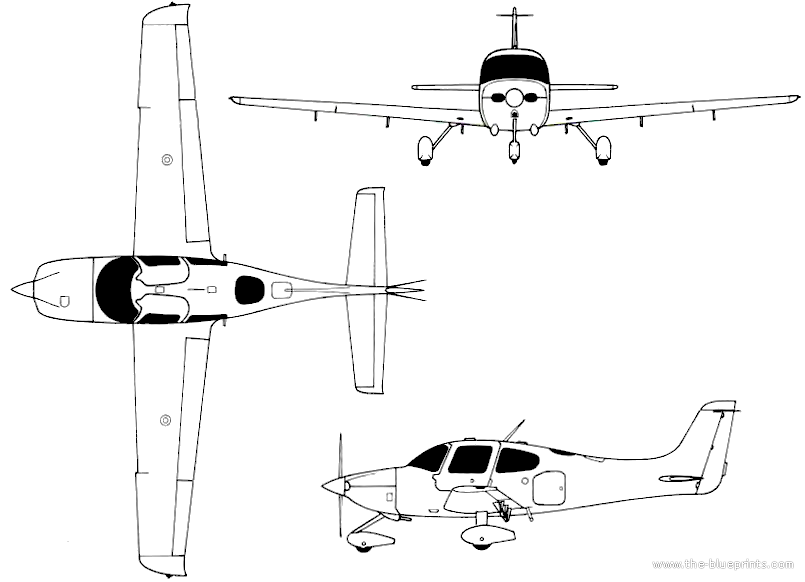
\includegraphics[width=0.4\textwidth]{imagens/blueprint.png}
  \caption{Três vistas do Cirrus SR22. Fonte:~\cite{blueprint_sr22}.}
  \label{fig:sr22}
\end{figure}

\begin{table}[H]
  \centering
  \caption{Principais características do Cirrus SR22. Envergadura, área alar e
  massa máxima (números de série 3915 e seguintes) segundo~\cite{easa_tcds};
  velocidade e Mach segundo~\cite{airplaneslist}; $Re$ calculado com a corda na
  raiz e a atmosfera padrão ao nível do mar~\cite{anderson}.}
  \label{tab:sr22}
  \begin{tabular}{lc}
    \toprule
    Parâmetro & Valor \\
    \midrule
    Envergadura $b$ [m]                         & 11,67 \\
    Área alar $S$ [m$^2$]                       & 13,46 \\
    Alongamento $AR = b^2/S$                    & 10,1 \\
    Corda na raiz / na ponta [m]                & $\approx 1{,}49$ / $0{,}89$ \\ % TODO: fonte das cordas
    Massa máxima à descolagem $W/g$ [kg]        & 1\,633 \\
    Velocidade de voo de referência $V_\infty$ [km/h] & 340 \\
    Número de Mach $M_\infty$                   & 0,28 \\
    Número de Reynolds $Re = \rho_\infty V_\infty c_r/\mu_\infty$ & $9{,}6\times10^{6}$ \\
    \bottomrule
  \end{tabular}
\end{table}

Na ausência das coordenadas do perfil do SR22, utilizou-se o perfil
Roncz/Marske-7 da base de dados da UIUC~\cite{uiuc_coord}, também associado a Roncz. A base de
dados descreve-o como um perfil de baixo arrasto para asa voadora, com
a linha média a descer abaixo da corda junto ao bordo de fuga. Sendo um perfil substituto, poderá não ser
representativo do perfil real do SR22. Como
$M_\infty \approx 0{,}28 < 0{,}3$, o escoamento pode ser considerado
incompressível~\cite{anderson}.
